\section{Experiment}

\subsection{Result Comparison}

\subsubsection{Comparison between categorical smoothing and Laplace smoothing}

\begin{table}[t]
\caption{Precision Comparison between categorical smoothing and Laplace smoothing}
\label{tab-smoothing-comparison}
\vskip 0.15in
\begin{center}
\begin{small}
\begin{sc}
\begin{tabular}{l|cc|c}
\hline
\abovespace\belowspace
Data set & Laplace & categorical & improvement \\
\hline
\abovespace
Top 1k set & 0.5906 & 0.8764 & 0.2858 \\
\belowspace
Lower 1k set & 0.6455 & 0.8128 & 0.1673 \\
\hline
\end{tabular}
\end{sc}
\end{small}
\end{center}
\vskip -0.1in
\end{table}

We use two different verb sets to compare the effect of categorical smoothing and Laplace smoothing. One set is the top 1000 most frequent unstemmed verbs in the SVO tuple corpus, the other lower 1000 set is the 10001st to 11000th most frequent unstemmed verbs in the SVO tuple corpus. The top 1000 set contains 538 unique stemmed verbs while the lower 1000 set contains 935 unique stemmed verbs. However, the number of examples in training and testing set are quite different. The top 1000 set has about 206k testing examples while the lower 1000 set has 18.9k testing examples. The numbers of training set have the same proportion.

From the comparison result in \ref{tab-smoothing-comparison}, we see that categorical smoothing provides a significant improvement on the precision on both datasets. It improves the precision on top 1000 set for 0.2858 and lower 1000 set for 0.1673 respectively. We also observe that the improvement of categorical smoothing is more significant on the top 1000 set than on the lower 1000 set.

\subsection{Comparison between Unigram Prior and Uniform Prior}

\begin{table}[t]
\caption{Precision Comparison between Unigram Prior and Uniform Prior}
\label{tab-prior-comparison}
\vskip 0.15in
\begin{center}
\begin{small}
\begin{sc}
\begin{tabular}{l|cc}
\hline
\abovespace \belowspace
Data set & Top 100 set & Lower 100 set \\
\hline
\abovespace
unigram prior & 0.8603 & 0.6376 \\
\belowspace
uniform prior & 0.9314 & 0.7784 \\
\hline
\abovespace
\belowspace
Difference & 0.0711 & 0.1408 \\
\hline
\end{tabular}
\end{sc}
\end{small}
\end{center}
\vskip -0.1in
\end{table}

\subsection{Smoothing Parameter}

\begin{figure}[ht]
\vskip 0.2in
\begin{center}
\centerline{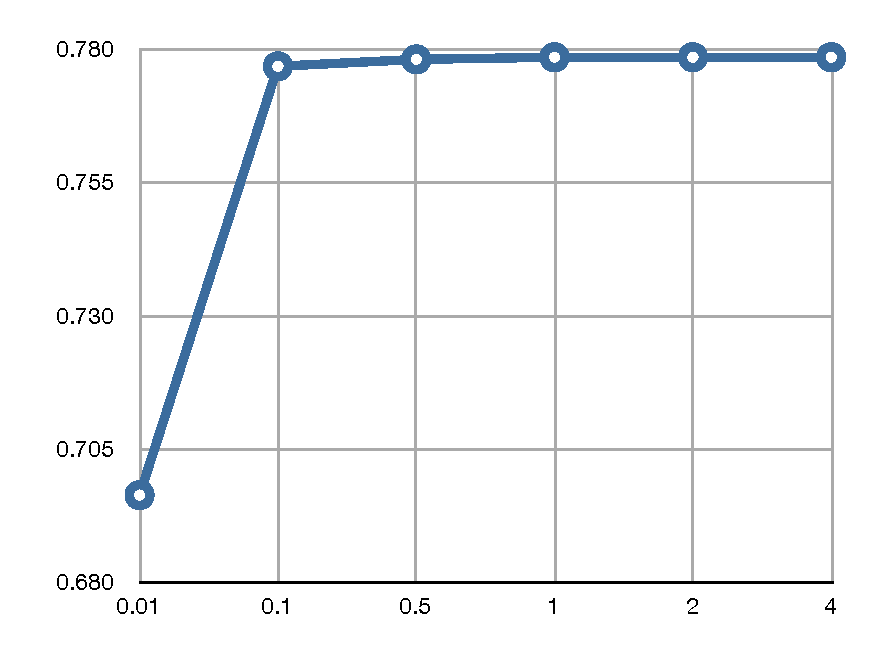
\includegraphics[width=\columnwidth]{pvsalpha}}
\caption{Precision vs. Smoothing parameter in Categorical Smoothing}
\label{fig-p-vs-alpha}
\end{center}
\vskip -0.2in
\end{figure}

We tuned the smoothing parameter $\alpha$ manually with several different values. When $\alpha$ is set to one, it is similar to Laplace smoothing but works on categorical counts instead of global vocabulary size. When $\alpha$ gets larger, the effect of category information is enlarged. From Figure \ref{fig-p-vs-alpha}, we find that when $\alpha$ is extreme small, the precision is decreased. When alpha increases, the precision generally increase, however, when alpha is larger than one, the precision is fixed on 0.7784 and never increases no matter how large it is set to.

We tried $\alpha=0$, and the experiment didn't success because of the zero probability product doesn't make sense. We tried to remove conditional probability of words and keep only the category based probability, but we got only a 0.0188 precision which is like random guess. We also had controlled experiments with Laplace smoothing with $\alpha=1$ and got the precision 0.6074, which is much lower than any alpha settings in categorical smoothing. 



